\part{Análisis estructurado}

\section{Introducción} % Revisar toda esta parte introductoria.
\paragraph{Modelo}
Descripción simplificada del sistema que se utiliza en análisis de requisitos como herramienta sobre la que trabajar con el cliente para construir un sistema adecuado a sus necesidades.

% Todos los métodos de análisis de requisitos se basan en la construcción de modelos del sistema que se pretende desarrollar

% \subsection{Ventajas}
% \begin{enumerate} %Esto se puede acortar
%     \item \textbf{Permite centrarse en las características más importantes del sistema}: Las discusiones con el cliente se centrarán en los aspectos más importantes del sistema.
%     \item \textbf{Permite realizar cambios y correcciones a los requisitos a bajo coste y sin correr ningún riesgo}: Si no se realizasen modelos, no se detectarían los fallos hasta después de construir el producto software.
%     \item \textbf{Permite verificar que el ingeniero del software ha entendido correctamente las necesidades del usuario}.
% \end{enumerate}

\subsection{Problemas del análisis clásico}
Consistía en redactar especificaciones funcionales, en forma de documentos de texto. \uline{Problemas}:
%La mayor parte de este problema es que la gente no modularizaba sus documentos... en fín.
\begin{enumerate}
    \item \textbf{Monolíticas}: Había que leerlos de principio a fin.
    \item \textbf{Redundantes}.
    \item \textbf{Ambiguas}: Causado por el uso del lenguaje natural.
    \item \textbf{Imposibles de mantener o modificar}: Al ser redundantes, cualquier modificación de una parte podía provocar una inconsistencia, obligando a leer todo el documento debido a que era una ``unidad monolítica''.
\end{enumerate}

\subsection{Soluciones al análisis clásico}
Surgieron \uline{nuevos métodos} de análisis para obtener especificaciones:

\begin{enumerate}
    \item \textbf{Gráficas}: comentadas, únicamente material de referencia. %Diagramas acompañados de información textual detallada.
    \item \textbf{Particionadas}: Facilitan la lectura de partes individuales de la especificación.
    \item \textbf{Mínimamente redundantes}.
    \item \textbf{Transparentes}: Fáciles de leer y comprender. %en ningún momento te dice que sean concisas ajjajajXD
\end{enumerate}


%Lo siento mucho almuiña pero aquí es probable que pregunte por siglas
\section{Técnicas de especificación y modelado}
El análisis estructurado \textbf{propone la descripción de los sistemas según 3 puntos de vista}:
\begin{enumerate}
    \item \textbf{Punto de vista de los datos (información)}: Información que utiliza el sistema, haciendo explícitas las relaciones entre datos.
          \begin{itemize}
              \item \textbf{D}iagramas \textbf{E}ntidad--\textbf{R}elación (\textbf{DER}).
              \item \textbf{D}iagramas \textbf{E}structura de \textbf{D}atos (\textbf{DED}).
          \end{itemize}
    \item \textbf{Punto de vista del proceso (función)}: Se centra en qué hace el sistema. Conjunto de operaciones de proceso de información.
          \begin{itemize}
              \item \textbf{D}iagramas de \textbf{F}lujo de \textbf{D}atos (\textbf{DFD}).
              \item Especificaciones de Procesos: termino genérico que engloba la definición de como un sistema transforma unas entradas en salidas mediante pseudocódigo, lenguaje natural, diagramas de flujo\ldots
          \end{itemize}
    \item \textbf{Punto de vista del comportamiento (tiempo)}: Se centra en cuándo sucede algo en el sistema. Sucesión de estados o modos de funcionamiento. Se indican las condiciones o eventos que hacen que el sistema pase de un modo a otro.
          \begin{itemize}
              \item Diagramas de Flujo de Control.
              \item Especificaciones de Control.
              \item Diagramas de Estados.
          \end{itemize}
\end{enumerate}

Utilizando estos modelos en conjunto podremos obtener una descripción detallada del \textbf{mismo sistema}.

% Habría que pensar un buen nombre para esta tabla
\begin{table}[ht]
    \centering
    \resizebox{\textwidth}{!}{
        \begin{tabular}{c|l|l|l|} \cline{2-4}
                                                                        & \multicolumn{1}{c|}{\textbf{Información}} & \multicolumn{1}{c}{\textbf{Función}} & \multicolumn{1}{|c|}{\textbf{Tiempo}} \\ \hline

            \multicolumn{1}{|c|}{\multirow{4}{*}{\textbf{Información}}} & D. entidad--relación                      &                                      &                                       \\
            \multicolumn{1}{|c|}{}                                      & D. de estructura de datos                 &                                      &                                       \\
            \multicolumn{1}{|c|}{}                                      & Matriz entidad/entidad                    &                                      &                                       \\
            \multicolumn{1}{|c|}{}                                      & Diagramas de clases                       &                                      &                                       \\ \hline

            \multicolumn{1}{|c|}{\multirow{7}{*}{\textbf{Función}}}     & D. de flujo de datos                      & D. de flujo de datos                 &                                       \\
            \multicolumn{1}{|c|}{}                                      & Matriz función/entidad                    & D. de casos de uso                   &                                       \\
            \multicolumn{1}{|c|}{}                                      & Diagrama de clases                        & D.de estructura de datos             &                                       \\
            \multicolumn{1}{|c|}{}                                      & D. de colaboración                        & Tarjetas CRC                         &                                       \\
            \multicolumn{1}{|c|}{}                                      &                                           & D. de componentes                    &                                       \\
            \multicolumn{1}{|c|}{}                                      &                                           & D. de despliegue                     &                                       \\
            \multicolumn{1}{|c|}{}                                      &                                           & D. de actividad                      &                                       \\ \hline

            \multicolumn{1}{ |c| }{\multirow{4}{*}{\textbf{Tiempo}}}    & H\textordfeminine\ de vida de la entidad  & Redes de Petri                       & D. de flujo de control                \\
            \multicolumn{1}{|c|}{}                                      & D. de estados                             & D. de estados                        & D. de estados                         \\
            \multicolumn{1}{|c|}{}                                      & D. de secuencia                           & D. de secuencia                      &                                       \\
            \multicolumn{1}{|c|}{}                                      &                                           & D. de actividad                      &                                       \\ \hline
        \end{tabular}
    }
    \caption{Métodos de modelado según la dimensión del sistema que modelan}
    \label{tab:nonametable}
\end{table}


\subsection{Diagramas de flujo de datos (DFD)}
Representa la programación desde un \textbf{punto de vista funcional}, esto es, las \textbf{entidades básicas son funciones o procesos} que transforman unos datos de entrada en salidas. El sistema se describe como el flujo de información a través de estas funciones.
\begin{enumerate}
    \item Las funciones del sistema.
    \item Las interacciones entre funciones: a dónde va la información de salida de una determinada función.
    \item Las transformaciones de datos del sistema: donde se almacena la información después de pasar por las funciones.
    \item Las transformaciones entrada--salida: por donde entra esa información \textbf{al sistema} y a dónde sale. % Qué datos de entrada se transforman en qué datos de salida. Reescrito : Las transformaciones entrada--salida
\end{enumerate}
Los DFD \textbf{NO} representan el \textbf{comportamiento}, sólo dicen lo que hace el sistema pero \textbf{NO} indican: %trasparrabas literales, pregunta de examen
\begin{enumerate}
    \item \textbf{Cuando se hace}.
    \item \textbf{En que secuencia se hace}.
\end{enumerate}


\subsubsection{Elementos}

%Imagen con la notación utilizada (mejor la estandar que sale en la wikipedia
\begin{figure}[H]
    \centering
    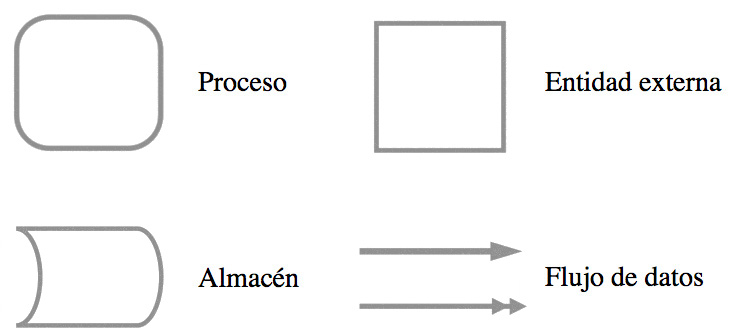
\includegraphics[width=0.5\linewidth]{Resources/elementosDFD}
    \caption{Notación estándar utilizada para representar los elementos del DFD.}
    \label{fig:elementosDFD}
\end{figure}
\begin{enumerate}
    \item \textbf{Procesos}: Representan elementos software que transforman información.

    \item \textbf{Entidades externas}: Representan elementos del sistema informático o de otros sistemas adyacentes que producen o consumen información transformada por el software. Los flujos de datos que comunican el sistema con las entidades externas representan las interfaces del sistema. \textbf{Sólo aparecen en el diagrama de contexto}.

    \item \textbf{Almacenes de datos}: Representan información almacenada que puede ser utilizada por el software. En la mayoría de los casos, utilizaremos almacenes de datos cuando los procesos intercambien información pero no estén sincronizados.

    \item \textbf{Flujos de datos}: Representan datos o colecciones de datos que fluyen a través del sistema. Conectan los procesos con otros procesos, con entidades externas o con almacenes de datos. Contienen información de las 3 dimensiones, aunque normalmente sólo representan las dimensiones de Función e Información.\\
          Según su \textbf{dimensión temporal}:
          \begin{enumerate}[a.]
              \item \textbf{Discretos}\textit{(Flecha con una cabeza)}: Representan movimiento de datos en un instante determinado de tiempo.
              \item \textbf{Continuos}\textit{(Flecha con con dos cabezas)}: Transmisión continua de información.
          \end{enumerate}
\end{enumerate}

%El rabo pone bastante incapié en los niveles y utiliza una nomenclatura confusa.
\subsubsection{Niveles}
Los \textbf{DFD} permiten la representación del sistema en múltiples niveles de abstracción, de esta forma se pueden representar gráficos con un número reducido de procesos (máximo 7$\pm$2). Deberíamos usar 7-8 niveles como mucho.
\begin{enumerate}
    \item \textbf{Nivel 0}: \textbf{Diagrama de Contexto}\\
          Representa el sistema como un único proceso, el \textbf{proceso 0}. Se representan también las entidades que interactúan con el mismo, dejando claro los \textbf{límites del sistema}.

          %Imagen nivel 0
          \begin{figure}[h!]
              \centering
              \includegraphics[width=0.45\linewidth]{Resources/niv-0}
              \caption{DFD de nivel 0 de un sistema.}
              \label{fig:dfdn0}
          \end{figure}
    \item \textbf{Nivel 1}: \textbf{Diagrama 0}\\
          Denominado así porque \textit{descompone el proceso 0} en sus funciones principales. Es interesante que éstas sean \textit{independientes} y que procesen \textit{las mismos flujos} que el de nivel 0.
          %Imagen nivel 1
          \begin{figure}[h!]
              \centering
              \includegraphics[width=0.45\linewidth]{Resources/nivel-1}
              \caption{DFD de nivel 1 de un sistema.}
              \label{fig:dfdn1}
          \end{figure}
    \item \textbf{Niveles 2\ldots $n-1$}\\
          Continuamos descomponiendo los procesos en subprocesos, recogiendo las interfaces (flujos) de nivel superior y asignándoselas a subprocesos.
          %Imagen nivel 2
          \begin{figure}[h!]
              \centering
              \includegraphics[width=0.45\linewidth]{Resources/nivel-2-p5}
              \caption{DFD de nivel 2 del proceso $5$ del sistema.}
              \label{fig:dfdn2}
          \end{figure}
    \item \textbf{Nivel $n$}\\
          Contiene los procesos primitivos, que no podemos descomponer. Si queremos describirlo debemos utilizar técnicas de especificación de procesos.
\end{enumerate}

Los procesos en el DFD tienen un \textbf{identificador numérico}:
\begin{enumerate}
    \item Nivel 0: solo tiene un proceso: el \textbf{``0''}
    \item Nivel 1: se le asigna a cada proceso un numero secuencialmente: \textbf{\{1, 2, 3\ldots\}}
    \item Nivel 2: a cada descomposición de cada proceso se le asigna un número secuencial después de un punto. Si descomponemos el \textit{proceso 1} en 3 tendríamos los procesos: \textbf{\{1.1, 1.2, 1.3\}}
    \item Niveles 2..N: a partir de aquí vamos concatenando la versión que descomponen con el número de secuencia \textbf{sin utilizar punto}. Descomponiendo el proceso \textit{1.1} en 2 tendríamos: \textbf{\{1.11, 1.12\}}
\end{enumerate}




\subsection{Especificaciones de proceso (PSPEC)} %Vaya mierda de definición original tenía esto
El \textbf{P}rocess \textbf{Spec}ification es un documento que describe textualmente los detalles de un proceso, indicando cómo es el proceso de transformación de una información de entrada en otra de salida.
\\
Debe ser \textbf{breve} (menor a una página) e incluir siempre \textbf{precondiciones} y \textbf{postcondiciones}.
\\
Para su elaboración, se utilizan diferentes \uline{técnicas de especificación}:

\begin{enumerate}
    \item Lenguaje natural.
    \item Diagrama de flujo.
    \item Lenguaje estructurado (Pseudocódigo).
    \item Arboles de decisión.
    \item Tablas de decisión.
\end{enumerate}
% traparaba de arbol de decisión y tabla de decisión


\subsection{Diagramas de flujo de control (DFC)}
Los \textbf{D}iagramas de \textbf{F}lujo de \textbf{C}ontrol (DFC) especifican todo el flujo de sucesos, señales y condiciones de datos del sistema.
\\
\\
%Traspa 37
Los DFC se crearon como diagramas complementarios de los DFD para suplir las carencias de los mismos:
\begin{itemize}
    \item \textbf{NO} representan el \textbf{procesamiento ni la transformación} de los flujos de control (eso se hace con las CSPECs).
    \item \textbf{NO} representan los \textbf{estados del sistema}.
\end{itemize}
Para solucionar esto el DFC añade las siguientes \uline{entidades}:
\begin{itemize}
    \item \textbf{Flujos de control}: información que determina si un proceso se activa o se detiene.
    \item \textbf{Almacenes de control}: Sirven para almacenar la información de control(estado del sistema)
    \item \textbf{Condiciones de datos}: Flujos de control generados por un proceso.
    \item \textbf{Ventanas de control}: (representadas por una barra) Indican el procesamiento de señales de control. Su comportamiento se define en las especificaciones de control (CSPEC).
    \item \textbf{Activadores de procesos} Señales de control especiales que activan o desactivan procesos tomando dos posibles valores: \texttt{ON} y \texttt{OFF}. Siguen la jerarquía de los modelos, es decir: un proceso está activo si y sólo si todos sus antecesores están activos.
          \\
          \textit{Por defecto: si no tiene activador, un proceso se considera activo si sus antecesores lo están}.
\end{itemize}

\begin{figure}[H]
    \centering
    \includegraphics[width=0.9\linewidth]{Resources/ejemploDFC}
    \caption{Ejemplo de un sistema de traducción. Préstese atención a las condiciones de dato: \textit{buffer lleno/buffer vacío}, las ventanas de control (barras) y el activador.}
    \label{fig:ejemploCSPEC}
\end{figure}


\subsubsection{Construcción de un DFC}
\begin{enumerate}
    \item Se elabora una jerarquía de DFCs paralela a la de los DFDs.
    \item Cada para DFC/DFD representa los mismos procesos y las mismas entidades externas.
    \item Sólo introducimos las señales de control que no estén implícitas en el DFD.
    \item A continuación, cada DFC se desarrollará en una especificación de control (CSPEC).
\end{enumerate}


\subsection{Especificaciones de control (CSPEC)}

El \textbf{C}ontrol \textbf{SPEC}ification es un documento que \textbf{especifica de manera secuencial o combinacional el comportamiento del programa}. Indicando bajo qué condiciones se emiten las señales de control que activan los procesos.
\\
\\
Existirá por lo tanto una \textbf{relación 1:1 entre los CSPEC y los DFC} de la jerarquía ya que el primero determina la activación del segundo, utilizando las \textbf{ventanas de control de los DFC como interfaces}.
\\
\\
% Especificación: división entre combinacional y secuencial.
Para su elaboración, se utilizan diferentes \uline{técnicas de especificación}:
\begin{enumerate}
    \item Lenguaje estructurado (Pseudocódigo). % parseo lo de la traspa
          \begin{figure}[h!]
              \centering
              \begin{verbatim}
                        SI BufferVacio
                            MIENTRAS NO BufferLleno
                                ESPERA Retardo
                                OnTimer
                            FIN MIENTRAS NO
                        FIN SI
  \end{verbatim}
              \caption{Ejemplo pseudocódigo para la activación de la función \emph{OnTimer}.}
          \end{figure}
    \item En sistemas combinacionales:
          \begin{itemize}
              \item Tablas de activación de procesos %parseo la de la traspa
                    \begin{table}[h!]
                        \centering
                        \begin{tabular}{|c|c|} \cline{1-2}
                                & MiraSiHayDatos \\ \hline
                            3.1 & 1              \\ \hline
                            3.2 & 0              \\ \hline
                            3.3 & 0              \\ \hline
                        \end{tabular}
                        \caption{Ejemplo de tabla de activación de un proceso.}
                    \end{table}


                    %Traspa 55
              \item Tablas de decisión
                    \begin{table}[h!]
                        \centering
                        \resizebox{0.4\textwidth}{!}{%
                            \begin{tabular}{|l|c|c|c|c|c|}
                                \hline
                                \multicolumn{6}{|c|}{\textbf{CONDICIONES}} \\ \hline
                                Condición 1 & Sí & Sí & No & No & No       \\
                                Condición 2 & Sí & -  & -  & -  & -        \\
                                Condición 3 & -  & Sí & -  & -  & -        \\
                                Condición 4 & -  & -  & Sí & -  & -        \\
                                            &    &    &    &    &          \\ \hline
                                \multicolumn{6}{|c|}{\textbf{ACCIONES}}    \\ \hline
                                Acción 1    & X  &    & X  &    &          \\
                                Acción 2    &    & X  &    & X  & X        \\\hline
                            \end{tabular}
                        }
                        \caption{Ejemplo de tabla de decisiones de un proceso.}
                    \end{table}
          \end{itemize}
    \item En sistemas secuenciales:
          \begin{itemize}
              \item Diagramas de estados
                    \begin{figure}[h!]
                        \centering
                        \includegraphics[width=0.9\linewidth]{Resources/estados}
                        \caption{Ejemplo de un diagrama de estados.}
                    \end{figure}

              \item Redes de Petri
                    \begin{figure}[H]
                        \centering
                        \includegraphics[width=0.9\linewidth]{Resources/redPetri}
                        \caption{Proceso de generación de una reclamación modelado en redes de Petri.}
                    \end{figure}
          \end{itemize}
\end{enumerate}





\subsection{Diagramas entidad--relación (DER)} % Mala definición
Los \textbf{D}iagramas \textbf{E}ntidad--\textbf{R}elación resuelven las insuficiencias que se pueden producir en la representación de los datos mediante los almacenes en los diagramas de flujo de datos (DFD), mostrando no sólo la información contenida si no las relaciones que existen entre los datos almacenados.

% no está en las traspas
% \subsection{Diccionario de datos (DD)} %No mal, quizás se pueda acortar un poquito la definición
% El diccionario de datos (DD) es un\textbf{ listado organizado de todos los elementos de datos que son pertinentes para el sistema, con definiciones precisas y rigurosas} que permiten que el usuario y el analista tengan una misma comprensión de las entradas, salidas, componentes de los almacenes y cálculos intermedios. Suele implementarse como parte de una herramienta CASE (Computer Aided Software Engineering) de análisis y diseño estructurados. El formato varía entre las distintas herramientas, pero \uline{suele contener}:
% \begin{itemize}
%     \item \textbf{ID}.%: Opcional.
%     \item \textbf{Nombre}: Único y descriptivo.%Nombre descriptivo único del elemento del almacén de datos o entidad externa.
%     \item \textbf{Alias}.%: Otros nombres.
%     \item \textbf{Dónde se usa/Cómo se usa}: Origen/Destino del flujo de datos, procesos que usan el dato y cómo lo usan.
%     \item\textbf{ Descripción del contenido}: Contenido representado según alguna notación.
%     \item \textbf{Comentarios adicionales}: Tipo de datos, valores implícitos, etc.
% \end{itemize}
% Una vez introducidos en el diccionario de datos un nombre y sus alias, se debe revisar la consistencia de las denominaciones.

% La información de dónde y cómo se usa un elemento se crea de modo automático a partir de la inspección de diagramas de control de flujo (DFC) y diagramas de flujo de datos (DFD). Mantener el diccionario de datos (DD) es extremadamente difícil para proyectos grandes, por eso las herramientas CASE son de gran ayuda. %Este párrafo creo que sobraba

\subsection{Comprobaciones a realizar sobre una especificación estructurada}
Debemos revisar si nuestra especificación cumple las siguientes propiedades.
\begin{enumerate}
    \item \textbf{Compleción}: Si los modelos son completos.
    \item \textbf{Integridad}: Si no existen contradicciones ni incoherencias entre modelos.
    \item \textbf{Exactitud}: Si los modelos cumplen los requisitos del usuario.
    \item \textbf{Calidad}: Estilo, legibilidad y facilidad de mantenimiento.
\end{enumerate}
\textit{Recomendación: checklist que compruebe a fondo que se cumplen estas propiedades}.



\subsection{Técnicas matriciales}
Las técnicas matriciales se utilizan \textbf{principalmente para ayudar a verificar la consistencia entre los componentes de distintos modelos} de un sistema.
\begin{enumerate}
    \item \textbf{Matriz entidad/función}: Visualiza las relaciones existentes entre las funciones que lleva a cabo un sistema y la información necesaria para soportarlas.\\
          Los elementos de las filas son entidades o relaciones presentes en el diagrama entidad--relación, mientras que los de las columnas pueden ser funciones de alto nivel representadas en un diagrama de flujo de datos.\\
          En cada celda se incluyen las \textbf{acciones} que puede realizar la función (\textbf{I}nsertar, \textbf{L}eer, \textbf{M}odificar y \textbf{B}orrar).
          %tabla pág 88 traparabas


          \begin{table}[h!]
              \centering
              \begin{tabular}{cl|c|c|c|} \cline{3-5}
                                                                                                          &                                   & \multicolumn{3}{c|}{\textbf{Funciones}}                              \\ \cline{3-5}
                                                                                                          &                                   & Gestionar Presupuesto                   & Gestionar Cliente & \ldots \\ \cline{2-5}
                  \parbox[t]{2mm}{\multirow{3}{*}{\rotatebox[origin=c]{90}{{\small \textbf{Entidades}}}}} & \multicolumn{1}{|c|}{Cliente}     & L                                       & I, M, B           &        \\ \cline{2-5}
                                                                                                          & \multicolumn{1}{|c|}{Presupuesto} & I, M, B                                 &                   &        \\ \cline{2-5}
                                                                                                          & \multicolumn{1}{|c|}{\ldots}      &                                         &                   &        \\ \cline{2-5}
              \end{tabular}
              \caption{Ejemplo de matriz entidad/función.}
              \label{tab:matrizEF}
          \end{table}

    \item \textbf{Matriz entidad/entidad}: Muestra las relaciones normales del diagrama entidad--relación.
          %tabla 89 traparaba
          \begin{table}[h!]
              \centering
              \begin{tabular}{cl|c|c|c|} \cline{3-5}
                                                                                                          &                                   & \multicolumn{3}{c|}{\textbf{Entidades}}                        \\ \cline{3-5}
                                                                                                          &                                   & Cliente                                 & Presupuesto & \ldots \\ \cline{2-5}
                  \parbox[t]{2mm}{\multirow{3}{*}{\rotatebox[origin=c]{90}{{\small \textbf{Entidades}}}}} & \multicolumn{1}{|c|}{Cliente}     &                                         & Tiene       &        \\ \cline{2-5}
                                                                                                          & \multicolumn{1}{|c|}{Presupuesto} &                                         &             &        \\ \cline{2-5}
                                                                                                          & \multicolumn{1}{|c|}{\ldots}      &                                         &             &        \\ \cline{2-5}
              \end{tabular}
              \caption{Ejemplo de matriz entidad/entidad.}
              \label{tab:matrizEE}
          \end{table}

          %mecago en dios tanto royo para definir señales de control y ahora usa eventos....
    \item \textbf{Matriz evento/entidad}: Muestra las acciones que provocan los eventos sobre las entidades: (\textbf{I}nsertar, \textbf{L}eer, \textbf{M}odificar y \textbf{B}orrar).
          %trapa raba 90
          \begin{table}[h!]
              \centering
              \begin{tabular}{cl|c|c|c|} \cline{3-5}
                                                                                                        &                                             & \multicolumn{3}{c|}{\textbf{Entidades}}                        \\ \cline{3-5}
                                                                                                        &                                             & Cliente                                 & Presupuesto & \ldots \\ \cline{2-5}
                  \parbox[t]{2mm}{\multirow{3}{*}{\rotatebox[origin=c]{90}{{\small \textbf{Eventos}}}}} & \multicolumn{1}{|c|}{Datos del cliente}     & I, M, B                                 &             &        \\ \cline{2-5}
                                                                                                        & \multicolumn{1}{|c|}{Datos del presupuesto} & I                                       & I, M, B     &        \\ \cline{2-5}
                                                                                                        & \multicolumn{1}{|c|}{\ldots}                &                                         &             &        \\ \cline{2-5}
              \end{tabular}
              \caption{Ejemplo de matriz evento/entidad.}
              \label{tab:matrizEvE}
          \end{table}
\end{enumerate}

\section{Metodología del análisis estructurado}

\subsection{Fases}

\begin{enumerate}
    \item Creación del modelo de procesos: Creamos los niveles de DFDs y las PSPEC.
    \item Creación del modelo de control: para cada DFD creamos un DFC y una CSPEC.
    \item Creación del modelo de datos: si los datos son complejos utilizamos un DER.
    \item Consistencia entre modelos: podemos hacer una lista de comprobación además de tablas para comprobar la coherencia.
\end{enumerate}

\subsection{Modelos complementarios}
Fuera de estas fases tenemos dos modelos más: %no lo tengo muy claro, parece así por las traspas
\begin{enumerate}
    \item \textbf{Modelo esencial o lógico}: es un modelo de lo que el sistema debe hacer para satisfacer los requisitos del usuario. En él no figura nada acerca de cómo se va a implementar el sistema, como los ficheros de backup, o la secuenciación de proceso.
    \item \textbf{Modelo de implementación}: En él se pueden mostrar detalles técnicos:
          \begin{itemize}
              \item Elección de dispositivos y formatos E/S.
              \item Volúmenes de datos, backups, dispositivos de almacenamiento.
              \item Tiempos de respuesta.
              \item Seguridad.
          \end{itemize}
\end{enumerate}
%Tema acabado

% El recorte más grande de los apuntes XD
% \subsection{Creación del modelo de procesos} % esto se puede poner fácilmente en pasos, sería mucho más legible. Hay paja.
% Mediante el uso de diagramas de flujos de datos (DFD) y especificaciones de proceso (PSPEC) podemos modelar el ámbito de información y ámbito funcional del sistema.
% %Lo dicho, poner en pasos estudio de la documentación inicial del sistema, análisis de la información de entrada y especifiación preliminar de componentes del sistema, elaboración del DFD de contexto…
% \\
% \\
% Antes de empezar a realizar diagramas, lo primero que tenemos que hacer es estudiar toda la documentación inicial del sistema, bien sea una especificación preliminar, o el resultado de reuniones con el cliente.
% \\
% \\
% Podemos analizar gramaticalmente la información de entrada, identificando los nombres (entidades externas, flujos y almacenes de datos) y verbos (procesos o funciones) de la especificación preliminar para identificar componentes del sistema.
% \\
% \\
% Comenzaremos por hacer el diagrama de flujo de datos (DFD) de contexto, mostrando el sistema en relación con las entidades externas con las que interactúa. A continuación, lo iremos refinando en mayores niveles de detalle. Hay que aplicar los principios de acoplamiento mínimo (máxima independencia) entre procesos distintos y máxima cohesión (fuerte conexión funcional entre todo lo que está dentro de un proceso) en cada proceso. El número de procesos por DFD debería estar entre 5 y 10. Al realizar descomposiciones, hay que mantener la consistencia de nombres, numeración y flujos de datos.
% \\
% \\
% No hay que caer en detalles de implementación, el DFD tan sólo debe mostrar una visión de cómo se mueve idealmente la información entre diferentes procesos.
% Según vamos incluyendo elementos en el DFD, hay que definirlos en el diccionario de datos (DD) del proyecto.
% \\
% \\
% Seguiremos descomponiendo hasta encontrar las primitivas de proceso, que serán procesos sencillos, con máxima cohesión. Los flujos de datos que entran y salen de las primitivas constituyen las interfaces de estos procesos. Describiremos estas primitivas mediante la especificación de proceso (PSPEC), a poder ser en pseudocódigo, manteniendo la consistencia de flujos de entrada y salida con respecto a los DFD.




% \subsection{Creación del modelo de control} %Esto también se debería poner en pasos
% No todos los sistemas necesitan un modelo de control, por lo que lo primero es determinar si es necesario o no.
% \\
% \\
% Si decidimos desarrollar un modelo de control, hay que establecer una jerarquía de diagramas de flujo de control (DFC) simétrica a la de DFD, donde cada par DFD/DFC contiene los mismos procesos, almacenes de datos y entidades externas, y en la misma posición.
% \\
% \\
% Eliminaremos del DFD todos los flujos que transporten información de control, para representarlos en los DFC. Hay que tener cuidado de no caer en detalles de implementación. En aquellos casos donde el comportamiento del sistema quede reflejado implícitamente en los DFD no haremos DFC.
% \\
% \\
% A cada par DFD/DFC le corresponde una especificación de control (CSPEC). Las condiciones de datos generadas por los procesos y las señales de control provenientes del exterior del DFC entrarán en las ventanas de control, de las que saldrán los activadores de procesos y las señales de control que salgan del DFC. Hay que mantener la consistencia de flujos de control entre las ventanas de control y las CSPEC.
% \\
% \\
% La especificación de control (CSPEC) puede ser combinacional, secuencial o compuesta. Las CSPEC combinacionales se representan mediante tablas de decisión y tablas de activación de proceso. Las secuenciales, mediante diagramas de estados.



% \subsection{Creación del modelo de datos}
% En el caso de que los datos por el sistema tengan una estructura compleja, se desarrollará a mayores de los Diccionarios de Datos (DD) un modelo de datos utilizando diagramas entidad--relación (DER).


% \subsection{Consistencia entre modelos}

% Una vez realizados los distintos modelos del sistema, se deberían llevar a cabo las técnicas de consistencia entre modelos. Dado que todos los modelos que podamos realizar representan el mismo sistema, deben de ser consistentes. Existen diversas \uline{reglas para asegurar la consistencia}:

% \begin{enumerate}
%     \item \textbf{Consistencia entre el modelo de procesos y el diccionario de datos}:
%     \begin{itemize}
%         \item Cada elemento de los diagramas de flujo de datos (DFD) debe estar definido en el diccionario de datos (DD).
%         \item Cada elemento del DD tiene que estar incluido en algún flujo de datos.
%     \end{itemize}
%     \item \textbf{Consistencia entre el modelo de control y el diccionario de datos}:
%     \begin{itemize}
%         \item Cada elemento de los diagramas de flujo de control (DFC) debe estar definido en el DD.
%         \item Cada señal de control definida en el DD tiene que estar incluido en algún flujo de control.
%     \end{itemize}
%     \item \textbf{Consistencia entre el modelo de datos y el diccionario de datos}:
%     \begin{itemize}
%         \item Los objetos y almacenes de datos del diagrama entidad--relación (DER) tiene que estar definidos en el DD.
%     \end{itemize}
%     \item \textbf{Consistencia entre el modelo de procesos y el modelo de datos}:
%     \begin{itemize}
%         \item Cada almacén de los DFD debe corresponderse con un objeto o relación del DER.
%         \item Los nombres de los elementos del DER y de los almacenes de los DFD tienen que corresponderse.
%         \item Las entradas del DD deben aplicarse tanto a los almacenes de datos como a los objetos y relaciones correspondientes.
%     \end{itemize}
%     \item \textbf{Consistencia entre el modelo de procesos y el modelo de control}
%     \begin{itemize}
%         \item Cada DFC y cada especificación de control (CSPEC) están asociados a un DFD. El recíproco no es necesariamente cierto. Los procesos, entidades externas y almacenes de datos del DFD deben aparecer en el DFC correspondiente.
%         \item Cada estado del diagrama de estados (DE se asocia a un proceso o grupo de procesos del DFD, activos durante ese estado, o al sistema esperando que se produzca algún evento.
%     \end{itemize}
%     \item \textbf{Consistencia plano información--función}
%     \begin{itemize}
%         \item Todos los elementos definidos en los DER deben estar definidos en el DD.
%         \item Todos los diagramas de estructuras de datos (DED) deben aparecer en el DD.
%         \item Cada entidad y relación del DER debe ser consultada y actualizada al menos una vez por alguna función primitiva del DFD.
%     \end{itemize}
%     \item \textbf{Consistencia plano información--tiempo}
%     \begin{itemize}
%         \item Cada entidad del DED debe tener asociado un diagrama de historia de la vida de las entidades (HVE).
%         \item Por cada entidad debe existir un evento que la crea.
%         \item Las HVE de las entidades maestro deben tratar las posibles repercusiones de
% borrar esa entidad sobre las entidades detalle.
%     \end{itemize}
%     \item \textbf{Consistencia tiempo--función}
%     \begin{itemize}
%         \item Debe existir un proceso primitivo dentro de los DFC que trate cada uno de los elementos identificados en la HVE.
%     \end{itemize}
% \end{enumerate}





% \section{Modelos del sistema: esencial y de implementación} % Demasiado texto, debe ser más conciso
% El modelo esencial del sistema \textbf{es un modelo de lo que el sistema debe hacer para satisfacer los requisitos del usuario}. En él no figura nada acerca de cómo se va a implementar el sistema. Es el resultado de la fase de análisis de requisitos del sistema.
% \\\\
% A partir del modelo esencial, los diseñadores podrían decidir cómo implementar el sistema, usando la tecnología disponible.
% \\\\
% Lo normal es que el cliente también decida sobre detalles de implementación, que formarán parte del \textbf{modelo de implementación}. El desarrollo del modelo de implementación está a caballo entre análisis y diseño. No puede ser desarrollado sólo por analistas y cliente porque se necesita consejo de diseñadores e implementadores, y no puede ser realizado sólo por diseñadores e implementadores porque el usuario debe definir una gran cantidad de requisitos de implementación, que irán surgiendo en la fase de análisis.
% \\\\
% El modelo de implementación será una \textbf{versión revisada y anotada del modelo esencial, donde se especifiquen todos los detalles adicionales proporcionados por el usuario}:

% \begin{enumerate}
%     \item \textbf{La elección de los dispositivos de entrada y salida}.
%     \item \textbf{La elección de los dispositivos de almacenamiento}.
%     \item \textbf{El formato de las entradas y salidas}%: Incluye el tamaño de los datos.
%     \item \textbf{La secuencia de operaciones de entrada y salida}%: Incluye la definición de cómo el sistema va a dialogar con el usuario.
%     \item \textbf{Volumen de datos}%: De esta forma se pueden prever las necesidades de procesamiento y almacenamiento.
%     \item \textbf{Tiempo de respuesta}.
%     \item \textbf{Copias de seguridad, y descarga de datos del sistema}%: Cuándo y de qué datos es necesario realizar una copia de seguridad. Mecanismos de recuperación. <- los mecanismos de recuperación van implícitos con los de copia de seguridad
%     \item \textbf{Seguridad}%: Mecanismos para evitar accesos no autorizados
% \end{enumerate}

% \subsection{Errores típicos al hacer modelos de sistema} % Esto se refiere a un esencial-> necesitamos reordenar con el anterior párrafo, dividir en subsecciones 
% \begin{itemize}
%     \item \textbf{Secuenciar de forma arbitraria los procesos del DFD}: El único secuenciamiento de funciones que debe aparecer en los DFD es el impuesto por la dependencia de datos.
%     \item \textbf{Utilizar ficheros temporales o de backup}%: Supuesta una tecnología perfecta, no serían necesarios, por lo que no son requisitos esenciales, sino de implementación.
%     \item \textbf{Utilizar información redundante}: Más en relación con la eficiencia de la implementación que con los requisitos del modelo.
%     %La definición de redundancia es redundante. Vaya, qué redundancia más redundante parece un documento de ENSO!
% \end{itemize}
